\section{Evaluation}
\label{sec.evaluation}


\begin{table*}[t]
\begin{tabular*}{\textwidth}{c @{\extracolsep{\fill}} rrrr}
%\begin{tabular}{lllr}
\toprule
\multicolumn{4}{c}{Kernel Footprint Generated by Running Apache} \\

%\multicolumn{1}{c}{\multirow{2}{*}{Powers} } &
\midrule
 & Native Linux    &  Lind & Graphene \\
\cmidrule(r){2-4}
& \multicolumn{3}{c}{Line Coverage} \\
\midrule
1. arch/x86/include/asm                 & 31.6\%          & 28.0\%    & 30.0\%      \\
2. arch/x86/include/asm/trace    &  10.0\%          & 0.0\%       &  5.0\%       \\
3. arch/x86/kernel                            &  22.8\%          & 19.5\%       & 15.2\%       \\
4. include/net                                     &  2.3\%            & 1.0\%       &  1.5\%          \\
5. drivers/cpuidle/governors         &  68.5\%          & 40.8\%       &  55.2\%       \\
\bottomrule
\end{tabular*}
\caption {Kernel Footprint Coverage}
\label{table:kernel_footprint_coverage}
\end{table*}


Our ultimate goal is to run legacy applications in Lind efficiently and securely. Especially, we want to demonstrate that by 
adopting our new ``safely re-implement'' model, Lind provides stronger security than existing systems using 
``check-and-pass-through'' or ``re-implement'' approaches. 


Through our evaluation, we want to show that:
\begin{itemize} 
  \item Legacy applications can run in Lind with acceptable overhead.
  \item Applications running in Lind can only trigger limited portion of the kernel and only touch commonly used kernel paths.   
  \item In Lind, the lines of code touched in the kernel are commonly used and not likely to trigger kernel bugs.   
\end{itemize}


\subsection{Performance Evaluation}

First, we have run different legacy applications in Lind to test performance overhead. Figure 3. shows the running time 
overhead of executing primes, grep and wget applications. 


\begin{figure}[h]
\centering
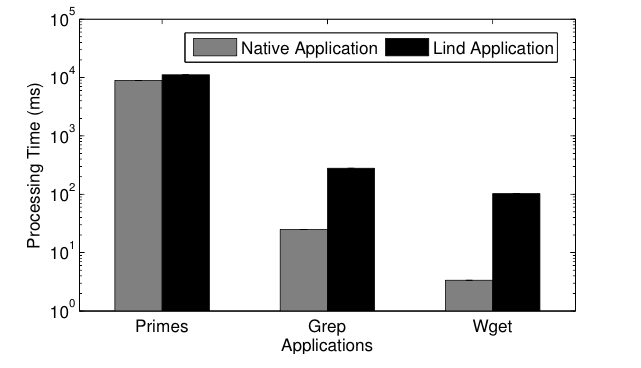
\includegraphics[width=1.0\columnwidth]{diagram/evaluation_01.png}
\caption{Primes, grep and wget performance: native vs. Lind}
\label{fig:arch}
\end{figure}


We have also run Tor in Lind and conducted measurement of performance overhead using Tor's built in benchmarks. 
The results are shown in Figure 4.


\begin{figure}[h]
\centering
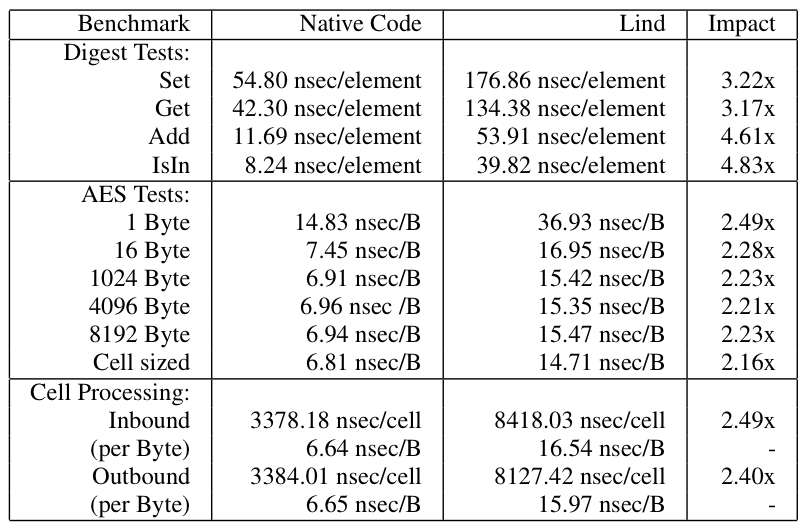
\includegraphics[width=0.9\columnwidth]{diagram/evaluation_02.png}
\caption{Results from Tor's built in benchmark program}
\label{fig:arch}
\end{figure}


To quantify the impact Lind has on memory use, we track how much memory Lind uses versus how much memory 
the same native program uses. Figure 5. shows the peak memory usage for each of the programs.

Lind's memory usage is actually very similar to the native programs, except for an relatively constant additional 
amount of memory (approximately 30 MB). That 30 MB is comprised of the additional overhead of running the NaCl 
sel\_ldr process to run the program, 


To summarize, the above experiments demonstrated that Lind was able to run applications with reasonable time and 
space overhead. Therefore, we believe Lind has the potential to become a widely deployed practical tool for 
common users. 


\begin{figure}[h]
\centering
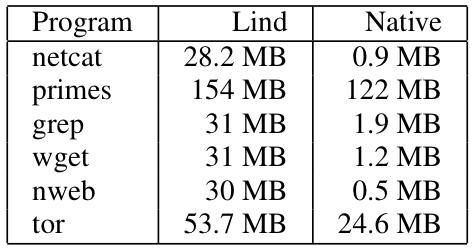
\includegraphics[width=0.6\columnwidth]{diagram/evaluation_03.png}
\caption{Memory consumption of programs running in Lind and natively.}
\label{fig:arch}
\end{figure}


\subsection{Security Evaluation}

In this security evaluation section, we would like to demonstrate the critical advantage of ``safely re-implement" model, 
and show how our design and implementation of Lind benefit from adopting this new isolation model. 
The essential advantages and benefits are better isolation between user applications and the kernel, and stronger 
protection of the kernel. 

The above advantages of Lind are demonstrated through the following facts, supported by our evaluation experiments:

\begin{itemize}  
  \item Only very limited portion of the kernel would be triggered and exposed.   
  \item The lines of code touched in the kernel are commonly used.  
  \item The kernel footprint generated by running applications in Lind is less likely to trigger kernel bugs. 
\end{itemize}

In addition, in order to show that Lind works better than existing system, in this security evaluation section, we also compared 
Lind against Graphene library OS system \cite{Graphene:14} to evaluate their security features. 


\subsubsection{Quantitative Analysis of the Kernel Footprint}

First of all, we want to examine the size of the kernel footprint generated by running applications under different environment.
To be specific, we ran legacy application, Apache, under: 

\begin{itemize} 
  \item Case 1: Native Linux OS
  \item Case 2: Lind
  \item Case 3: Graphene
\end{itemize}

We have quantitatively evaluated the size of the reachable kernel triggered by running applications in both Lind and Graphene, 
and under native linux OS.

The results for running Apache under the three different environment are illustrated in Table \ref{table:kernel_footprint_coverage} 
(speculative data).
 
In this experiments, we choose critical kernel paths and compare the coverage of kernel code under three different 
environment.
As shown from the results, we can learn that for those critical kernel paths, Lind covers only limited portion of the kernel code, 
significantly smaller than the code coverage under native Linux system. This demonstrates that Lind has minimum contact 
with the kernel while running complex legacy applications. Therefore, Lind provides better isolation between untrusted user 
applications and the privileged kernel. 


\subsubsection{Further Analysis of Kernel Footprint Composition}

In the previous subsection, we have quantitatively evaluated the size of kernel footprint generated by running applications 
under native Linux OS, Lind, and Graphene. We have shown that Lind touched the smallest portion of the kernel. 
Next, we want take one step further to closely examine the exact composition of the kernel footprint being touched. 

When we look at the kernel code/path, we can see they are used by different functions and are triggered with 
different frequencies. 
In order to reflect the above differences to help understand how different parts of the kernel have different influences 
over security,
we first define two critical terms important to our evaluation, ``common path'' and ``abnormal path''.

\begin{itemize} 
  \item Common path: parts of the kernel that are commonly used by popular packages and applications with good reputation. 
  \item Abnormal path: parts of the kernel that are rarely triggered by normal program behavior and are triggered 
  by reported kernel vulnerabilities. 
\end{itemize}

The purpose of defining those two terms is to help us better understand what kind of kernel code has been triggered 
under different environments, and therefore better perceive different degrees of security guarantee brought by 
implementing different isolation models. 


\begin{table}
\begin{tabular}{cc}
\toprule
\multicolumn{2}{c}{Packages \& Functions Used to Define ``Common path''} \\

\midrule
Linux Packages    &  Functions \\
\midrule
Readline & Open \\
Curl & Close \\
Zlib & Read \\
Binutils & Write \\
Automake & Mkdir \\
GMP & \\
Gzip & \\
Db & \\
Httpd & \\
Coreutils & \\
APR & \\
Make & \\
... & \\

\bottomrule
\end{tabular}
\caption {Packages \& Functions Used to Define ``Common path''}
\label{table:common_path}
\end{table}


``Common path'' in the kernel represents the safer parts of the kernel. Being frequently triggered by normal program behavior 
and benign code, the well-wore ``common path'' is less likely to cause security flaws and therefore can be trusted to allow 
contact with user applications. To define ``common path'', in our experiments, we selected 20 Linux packages and 5 basic 
functions that are popular and have good reputation (Shown in Table \ref{table:common_path}). We ran those packages and 
functions in Linux OS, and use Gcov to profile the kernel path touched. The kernel paths touched by running our packages and 
functions are considered ``common path''. 

``Abnormal path'' in the kernel represents corner cases and potential design flaws. Those paths cannot be reached by 
normal actions, while might be triggered by misconfiguration of flags and arguments, or malicious code trying to 
gain control of the system.  

To define ``abnormal path'', we examined 19 severe kernel bugs (Shown in Table \ref{table:abnormal_path}). 
We closely studied the kernel paths that are involved in triggering those bugs. The kernel paths that might potentially 
trigger the kernel bugs are considered ``abnormal path''. 


\begin{table*}[t]
\begin{tabular*}{\textwidth}{l @{\extracolsep{\fill}} lc}
\toprule
\multicolumn{2}{c}{Kernel Vulnerabilities Used to Define ``Abnormal path''} \\

\midrule
Vulnerability    &  Specific Type \\
\midrule
 CVE-2009-3234 \cite{CVE:20093234} & stack and heap buffer overflows \\
 CVE-2013-1828 \cite{CVE:20131828} & stack and heap buffer overflows \\
 CVE-2013-2892 \cite{CVE:20132892} & stack and heap buffer overflows \\
 CVE-2005-0736 \cite{CVE:20050736} & NULL pointer and pointer arithmetic errors \\
 CVE-2009-2698 \cite{CVE:20092698} & NULL pointer and pointer arithmetic errors \\
 CVE-2009-3002 \cite{CVE:20093002} &  memory disclosure vulnerabilities \\
 CVE-2010-4073 \cite{CVE:20104073} &  memory disclosure vulnerabilities \\
 CVE-2013-2852 \cite{CVE:20132852} &  use-after-free and format string bugs \\
 CVE-2013-4343 \cite{CVE:20134343} &  use-after-free and format string bugs \\
 CVE-2010-3437 \cite{CVE:20103437} &  signedness errors \\
 CVE-2013-2094 \cite{CVE:20132094} &  signedness errors \\
 CVE-2005-0736 \cite{CVE:20050736} &  integer overflows \\
 CVE-2010-2959 \cite{CVE:20102959} &  integer overflows \\
 CVE-2009-1527 \cite{CVE:20091527} &  race conditions \\
 CVE-2009-3547 \cite{CVE:20093547} &  race conditions \\
 CVE-2010-3904 \cite{CVE:20103904} &  missing authorization checks and poor argument sanitization\\
 CVE-2010-4347 \cite{CVE:20104347} &  missing authorization checks and poor argument sanitization\\
 CVE-2012-0946 \cite{CVE:20120946} &  missing authorization checks and poor argument sanitization\\
 CVE-2013-0268 \cite{CVE:20130268} &  missing authorization checks and poor argument sanitization\\

\bottomrule
\end{tabular*}
\caption {Kernel Vulnerabilities Used to Define ``Abnormal path''}
\label{table:abnormal_path}
\end{table*}


Now that we have defined ``common path'' and ``abnormal path'' in the kernel, we then use those two terms to 
categorize the kernel footprint generated under native Linux OS, Lind, and Graphene. We want to see the difference 
and what that means. 

In this experiment, the kernel footprint was generated by running Apache, GNU Wget and GNU Grep under 
native Linux OS, Lind, and Graphene. 

The kernel footprint composition results are shown in Table \ref{table:kernel_footprint_composition} (speculative data).  
Through the results, we can see that running applications in Lind touched ``common path'' nearly all the time, 
while ``abnormal path'' was triggered frequently under the other two environments, native Linux OS and Graphene. 
By the definition of ``common path'' and ``abnormal path'', our results indicate that Lind provides stronger protection 
to the OS kernel. 
  
In the next section, we will take one step further to verify that reported kernel vulnerabilities are indeed not likely 
to be triggered by running applications in Lind, while having more chances to be triggered under 
native Linux OS or Graphene. 


\begin{table}
\begin{tabular}{lccc}
\toprule
\multicolumn{4}{c}{Kernel Footprint Composition} \\
\midrule
 & Native Linux    &  Lind & Graphene \\
\cmidrule(r){2-4}
& \multicolumn{3}{c}{Composition Percentage} \\
\midrule
``Common path''     &   72.5\%      & 95.5\%    & 78.0\%      \\
``Abnormal path''    &  27.5\%      & 4.5\%       & 22.0\%       \\
\bottomrule
\end{tabular}
\caption {Kernel Footprint Composition}
\label{table:kernel_footprint_composition}
\end{table}


\subsubsection{Analysis of Previous Kernel Bugs}

In this section, we want to verify how likely it is to trigger kernel bugs under native Linux OS, Lind, and Graphene.
We will achieve our goal through conducting the following steps: \\

\begin{itemize}
  \item 1) Examine a list of 19 reported kernel bugs, and identify the kernel paths involved in triggering each of the bugs.
  \item 2) Generate kernel footprint by running Apache, GNU Wget and GNU Grep under native Linux OS, Lind, and Graphene. 
  \item 3) Match kernel footprint in 2) against kernel paths in 1) to verify if a bug can be triggered under each environment. 
\end{itemize}

The results for verifying which kernel bugs may be triggered under each environment is illustrated in Table 
\ref{table:trigger_vulnerabilities} (speculative data). 

Through the results, we can see the kernel footprint generated in Lind is the safest, 
since it triggers the least number of kernel bugs.

\begin{table*}[t]
\begin{tabular*}{\textwidth}{l @{\extracolsep{\fill}} ccc}
\toprule
\multicolumn{4}{c}{Possibility of Triggering Kernel Vulnerabilities} \\

\midrule
Vulnerability    &  Native Linux OS  &  Lind  &  Graphene \\
\midrule
 CVE-2009-3234 \cite{CVE:20093234} & yes & no & no \\
 CVE-2013-1828 \cite{CVE:20131828} & no & no & yes \\
 CVE-2013-2892 \cite{CVE:20132892} & yes & no & yes \\
 CVE-2005-0736 \cite{CVE:20050736} & yes & yes & yes \\
 CVE-2009-2698 \cite{CVE:20092698} & yes & no & yes \\
 CVE-2009-3002 \cite{CVE:20093002} & yes & no & yes \\
 CVE-2010-4073 \cite{CVE:20104073} & yes & no & yes \\
 CVE-2013-2852 \cite{CVE:20132852} & yes & no & no \\
 CVE-2013-4343 \cite{CVE:20134343} & yes & no & no \\
 CVE-2010-3437 \cite{CVE:20103437} & no & no & no \\
 CVE-2013-2094 \cite{CVE:20132094} & no & no & yes \\
 CVE-2005-0736 \cite{CVE:20050736} & no & no & yes \\
 CVE-2010-2959 \cite{CVE:20102959} & yes & no & yes \\
 CVE-2009-1527 \cite{CVE:20091527} & yes & no & yes \\
 CVE-2009-3547 \cite{CVE:20093547} & yes & no & yes \\
 CVE-2010-3904 \cite{CVE:20103904} & yes & no & no \\
 CVE-2010-4347 \cite{CVE:20104347} & no & no & yes \\
 CVE-2012-0946 \cite{CVE:20120946} & yes & no & no \\
 CVE-2013-0268 \cite{CVE:20130268} & yes & no & yes \\

\bottomrule
\end{tabular*}
\caption {Possibility of Triggering Kernel Vulnerabilities (``yes'': possible to trigger the bug; ``no'': not possible to trigger the bug)}
\label{table:trigger_vulnerabilities}
\end{table*}


\subsubsection{Conclusion}

The above three sets of experiments (in \S4.2.1, \S4.2.2, and \S4.2.3) conclude our security evaluation. 
Through the results, we have shown the security strengths of Lind and the merits of adopting 
the ``safely-reimplement'' model. 


